\documentclass{article}
\title{Project 2 Proposal}
\author{Guilherme Serpa}

\usepackage{graphicx}

\begin{document}

\maketitle
\centerline{Guilherme Serpa - 82078}
\centerline{Group 10}

\newpage{}
Original Document\\\\
For this project I am proposing to create a scene with several meshes. The first mesh is a
cube made of glass material and, as such, it is transparent and refractive. The other mesh is
a solid black sphere which is non-reflective (like a mirror) and non-refractive.
These 2 meshes will be put together to create a die (1 cube and the black sphere gets repeated
several times).

The scene will have a camera orbiting around it allowing the viewer to inspect the scene, zooming
in on the object and rotating around it.

The user will have the ability to take a snapshot of the openGL window/scene to a known image format
and if there is time, "photorealistic" lighting will be added in the form of Phong lighting.

Refraction is a shader based special effect with normals.

The scene should contain a skybox as well.

The technical challenges are therefore as such: \\
- [2.0] Generic scene graph. \\
- [1.0] Saving a snapshot of the application to a known image file format. \\
- [2.0] Non physically-based "photorealistic" lighting. \\
- [4.0] Realistic or stylised material with transparencies. \\
- [3.0] Shader based special effects. \\

An example of the intended result:\\
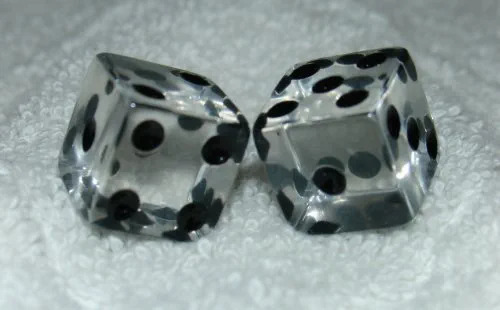
\includegraphics[scale=0.5]{dice.jpg} \\

Note: this image does not belong to me and was taken from an Amazon listing. \\
https://www.amazon.com/Vintage-Dice-Clear-Transparent-Pair/dp/B000UPTRIQ \\
The brand is called "Vintage Dice" and all rights belong to that entity. \\\\

The planned skybox is different from what is displayed in the image.

\newpage{}
Updated Document for Final Submission\\\\
I begun the project by creating the scene graph. To start off I needed simple VAO
and VBO creation using vertices input manually as a vector. 
\\With the VBOs and VAOs
working I created a function that would import objects from Blender, initially working 
wihout indices. With the object loading function complete I needed to make a function
for loading cubemaps/textures so for a while I worked on that.
When I finished that function I could also finish the skybox so I imported a cube and
applied the texture to the cube, did the matrices for it and had a working skybox.
\\Afterwards I worked on taking a snapshot of the application. I decided to use the
.ppm image format because it is very simple to work with. To create the file we just have
to write the header and then each RGB value in the scene. Following that I imported another cube, created a different set of shaders for it
and over several days worked on transparency and refraction in the shaders for that 
cube.
\\When I finally finished getting the refraction working properly, it was time to
use indices when importing objects because transparency was showing the object's 
triangles. Now that object importing was complete, I went back to Blender to create a "rounded"
cube for the dice. Created the object and imported it to the project.
\\Created the input handling for zooming in and out and rotating the scene. 
Created a sphere in Blender as well and imported it to the project. Scaled and
translated it to its correct position and used the VAO several times to create all
other dots/spheres on the die. Duplicated the first die and rotated it next to the first die. 
And at the end I added the capability to switch between 3 different skyboxes using the
1, 2, and 3 keys.
\\Photorealistic lighting was not implemented as it was not necessary for the required points.
\\In the end this was the final result: \\
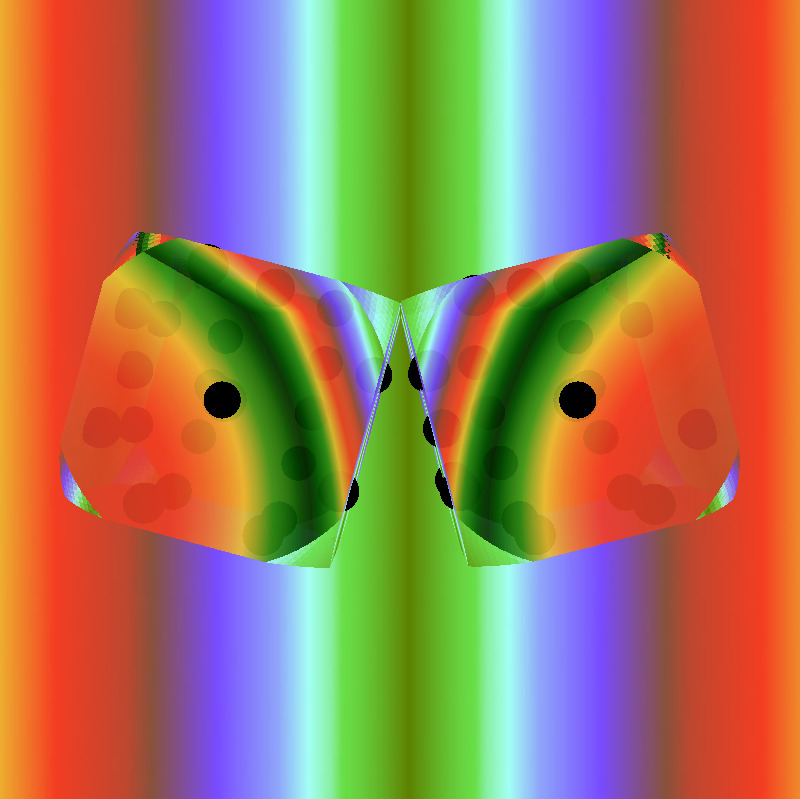
\includegraphics[scale=0.22]{result.jpg}
\end{document}
